% !TeX root = ../main.tex
% !TEX spellcheck = en_GB

\chapter{Architecture}
\label{sec:Architecture}
This section describes the overall system architecture, the chosen platforms for development and how the different subsystems communicate with each other.

\begin{figure}[H]
	\centering
	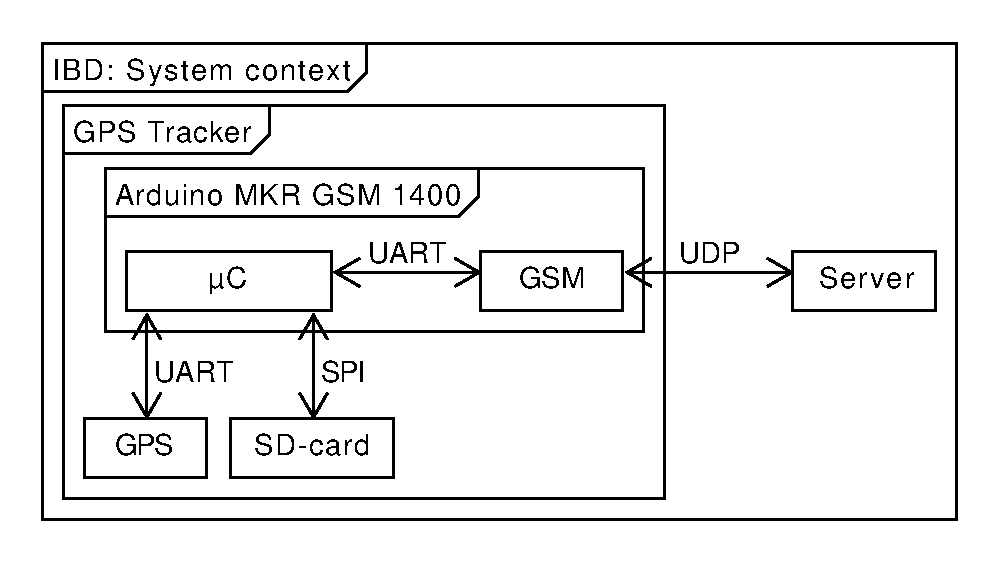
\includegraphics[width=0.7\linewidth]{gfx/Design/Overall_IBD.pdf}
	\caption{Overall BDD, including types of connection.}
	\label{fig:BDD:overall}
\end{figure}

\section{Choice of components}
The physical entities necessary to solve the tasks of the blocks identified in \cref{fig:BDD:unspecified} are as follows:

\paragraph{Controller and Data transfer} can be performed by a single module. The \MKR which includes a \SAMD ARM µC and a u-blox SARA-U201-03B-00 High Speed Packet Access (HSPA) with 2G fallback module for internet access.
They communicate using one of the two UARTs available on the \SAMD ARM µC.
The \SAMD ARM µC uses \SI{< 15}{\milli\ampere} while running \cite[p.~791-794]{SAMD21}.
The SARA-U201 uses a maximum of \SI{1.9}{\ampere} when transferring data \cite[p.~26]{SARAU201} and less than \SI{1}{\milli\ampere} when in power-saving mode.

\paragraph{Locator} has to be able to locate itself globally. This is solved using a GNSS module, u-blox NEO-7M-0-000, from Embedded Stock.
The module is able to use GPS (with SBAS and QZSS) and GLONASS, allowing for global positioning.
It also uses a maximum of \SI{67}{\milli\ampere} \cite[p.~17]{NEO7_Data} and is the low power version from the NEO-7 series.
The breakout-board exposes the UART connection, which can be used to communicate with the controller.

\paragraph{Memory} has to be non-volatile and able to store at least 1440 locations.
This is accomplished using a SD-card with \SI{2}{\giga\byte} of memory, allowing for each location to be up to \SI{1.39}{\mega\byte}.
The connection to the SD-card breakout board is SPI which is directly available on the \MKR module.

\section{Communication}
With the chosen components, the interfaces between them can be identified, as shown in \cref{fig:IBD:overall}.
The communication between the \SAMD and the \SARA module are presoldered to UART.
The breakout-board for the NEO-7M exposes UART ports and the SD-card breakout-board exposes SPI ports.
Connection to the server is chosen to be UDP with an acknowledge from the server.

\begin{figure}
	\centering
	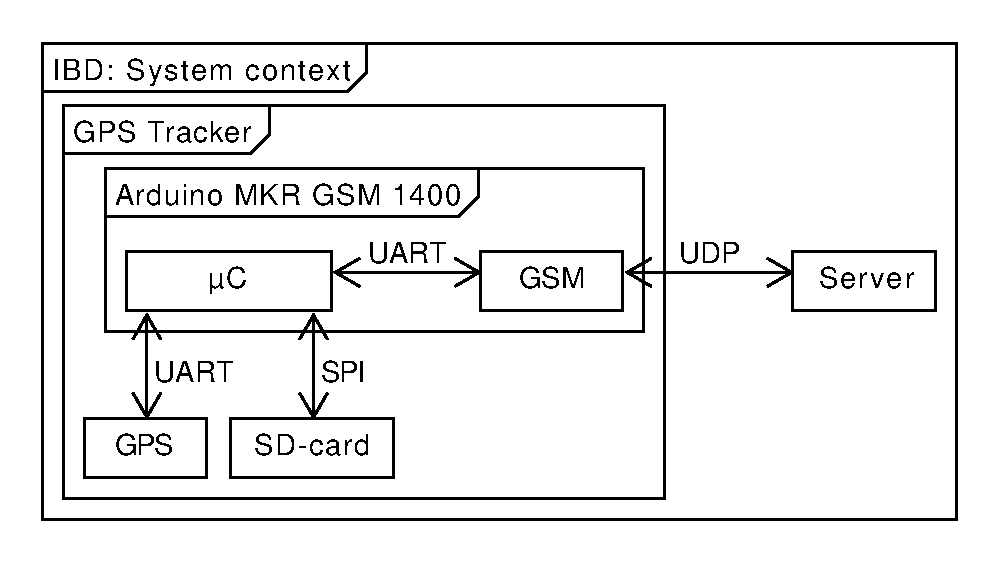
\includegraphics[width=0.7\linewidth]{gfx/Design/Overall_IBD.pdf}
	\caption{}
	\label{fig:IBD:overall}
\end{figure}


\section{Sequence Diagrams}

\begin{figure}
	\centering
	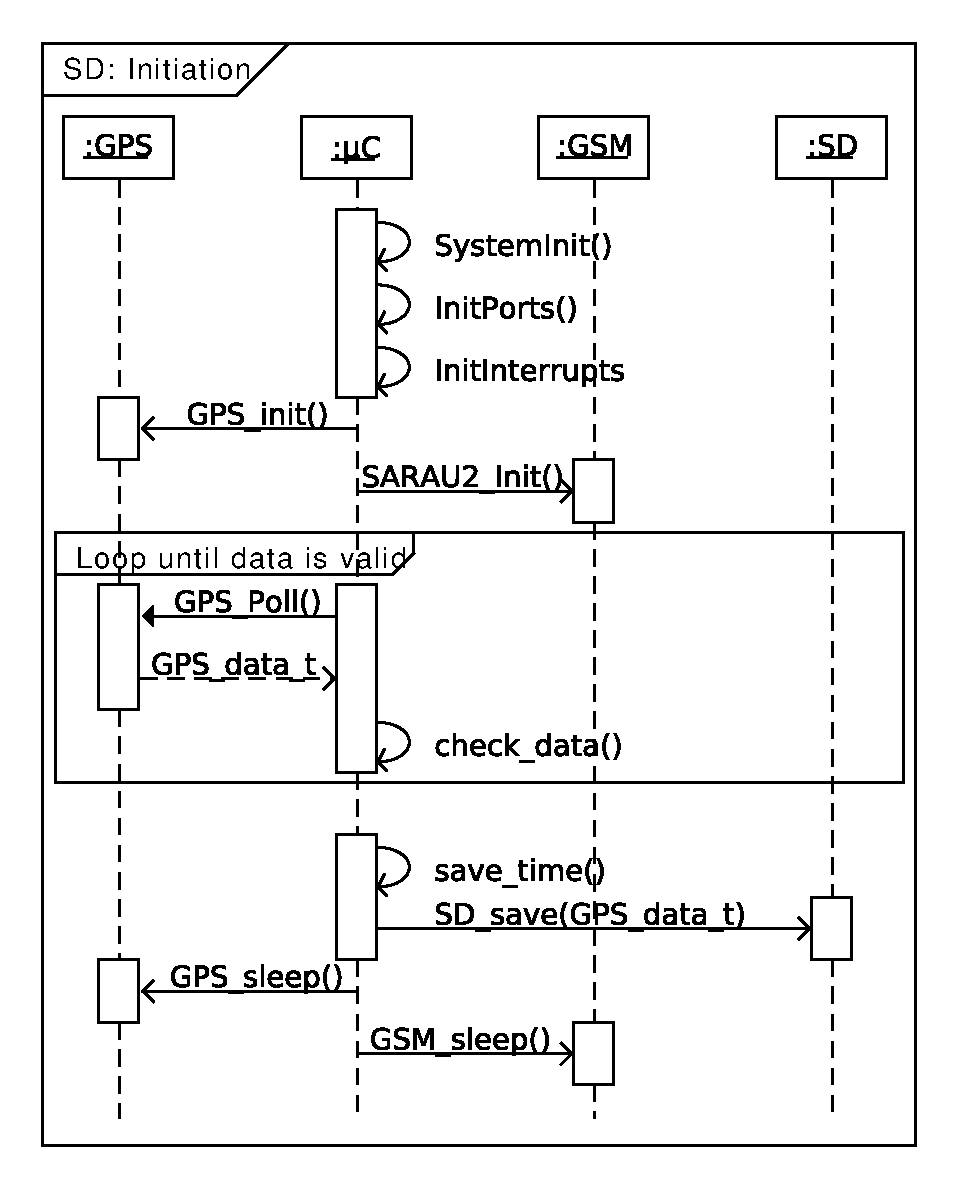
\includegraphics[width=0.7\linewidth]{gfx/Design/SD_init.pdf}
	\caption{}
	\label{fig:SD:init}
\end{figure}

\begin{figure}
	\centering
	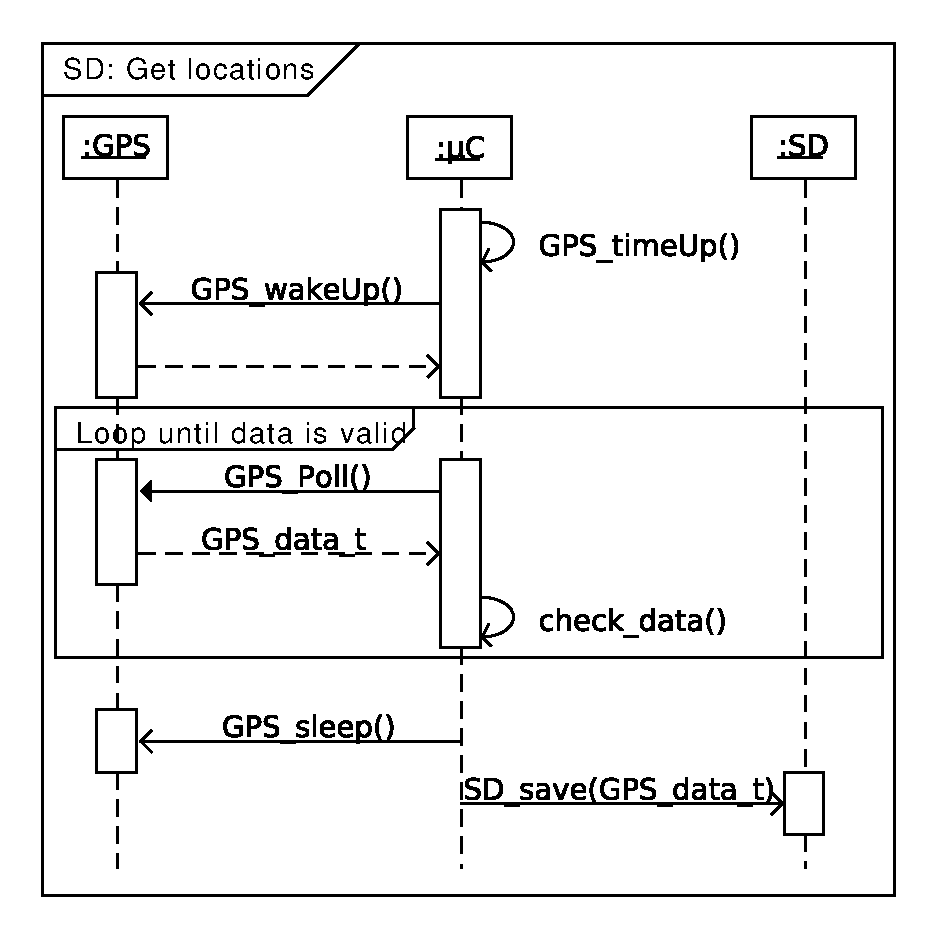
\includegraphics[width=0.7\linewidth]{gfx/Design/SD_getLocation.pdf}
	\caption{}
	\label{fig:SD:getlocation}
\end{figure}

\begin{figure}
	\centering
	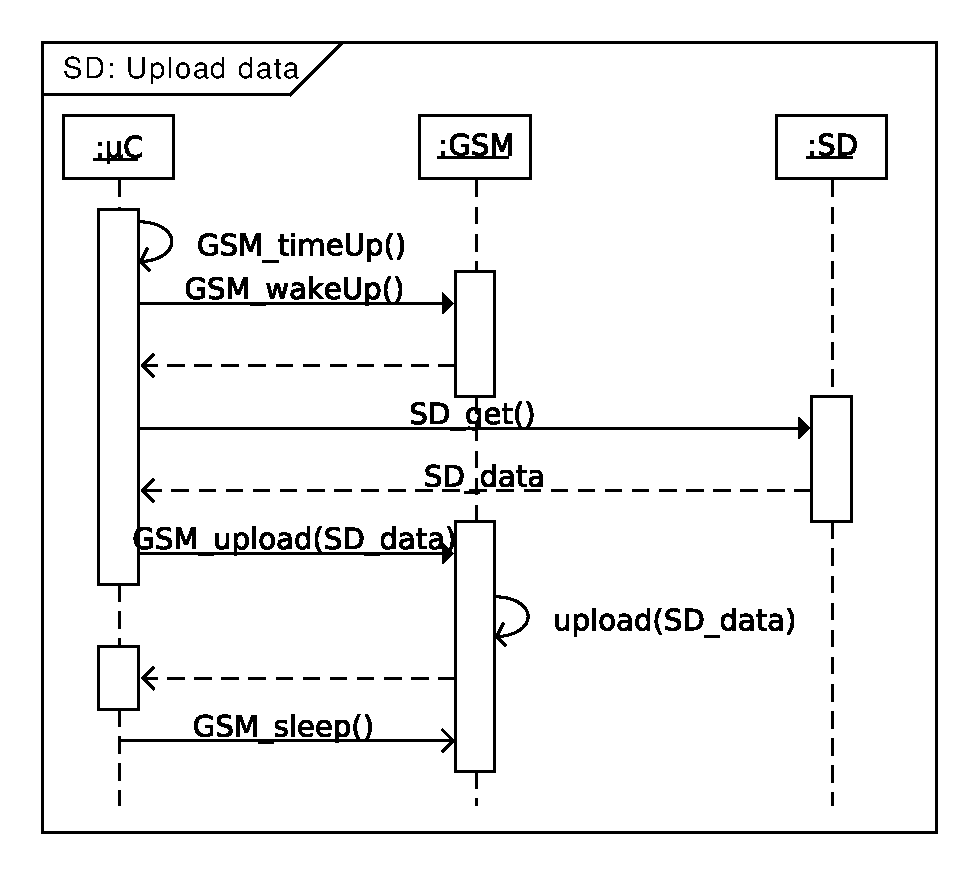
\includegraphics[width=0.7\linewidth]{gfx/Design/SD_Upload.pdf}
	\caption{}
	\label{fig:SD:upload}
\end{figure}



\FloatBarrier